\begin{figure*}[t]
\centering
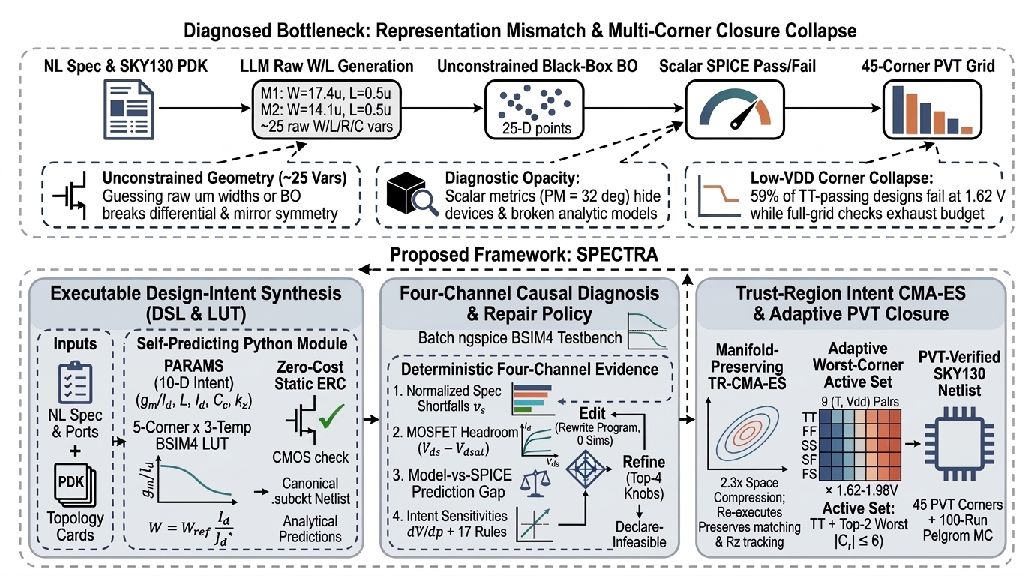
\includegraphics[width=0.98\textwidth]{figs/spectra_framework.pdf}
\vspace{-2.5mm}
\caption{Architecture of \textsc{SPECTRA}. Given a natural-language circuit specification and shared PDK/topology cards, \textbf{(a)} the LLM synthesizes an executable Python design-intent program that queries pre-characterized SKY130 BSIM4 lookup tables (\texttt{lut.size}) across 5 corners and 3 temperatures to emit both a canonical \texttt{.subckt} netlist and analytical self-predictions; \textbf{(b)} a static electrical-rule checker (ERC) filters illegal topologies at zero simulation cost before batch \texttt{ngspice} testbenches extract all target metrics; \textbf{(c)} a four-channel causal analyzer extracts normalized violations, device operating-region margins ($V_{DS}-V_{dsat}$), prediction-to-simulation discrepancies, and finite-difference intent sensitivities to steer a hierarchical policy (\textsc{Edit}, \textsc{Refine}, or \textsc{Declare-Infeasible}); and \textbf{(d)} bounded trust-region CMA-ES searches the low-dimensional intent space while preserving matching and bias invariants, closing 45-condition PVT targets via adaptive worst-corner promotion.}
\Description{System architecture diagram of SPECTRA showing four connected stages: executable design-intent program synthesis with BSIM4 lookup tables, static ERC and ngspice testbench evaluation, four-channel device-level causal diagnosis with hierarchical repair routing, and trust-region intent-space CMA-ES with adaptive 45-corner PVT verification.}
\label{fig:overview}
\end{figure*}
